\documentclass[border=3pt]{standalone}
\usepackage{tikz}
\usetikzlibrary{arrows.meta,calc}
\tikzset{pin/.style={-{Stealth[length=5pt]}},
  blk/.style={draw, thick, minimum width=18mm, minimum height=24mm, font=\sffamily}}
% bus slash with width label
\newcommand{\busslash}[2]{\draw ($#1+(-1mm,-1mm)$) -- ($#1+(1mm,1mm)$); \node[font=\scriptsize] at ($#1+(2mm,2mm)$){#2};}
\begin{document}
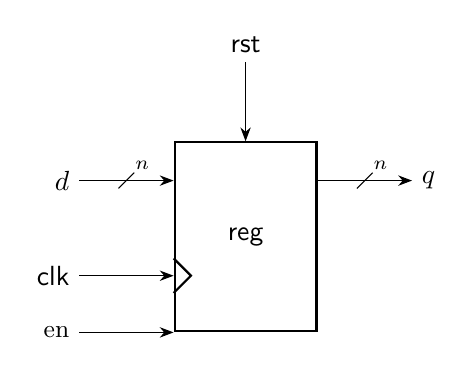
\begin{tikzpicture}[font=\sffamily]
  \node[blk] (r) {reg};
  % clock triangle, lower-left
  \draw[thick] ($(r.south west)+(0,5mm)$) -- ++(2.2mm,2.2mm) -- ++(-2.2mm,2.2mm);
  % data in (bus)
  \draw[pin] ($(r.north west)+(-12mm,-5mm)$) node[left]{$d$} -- ($(r.north west)+(0,-5mm)$);
  \busslash{($(r.north west)+(-6mm,-5mm)$)}{$n$}
  % data out (bus)
  \draw[pin] ($(r.north east)+(0,-5mm)$) -- ++(12mm,0) node[right]{$q$};
  \busslash{($(r.north east)+(6mm,-5mm)$)}{$n$}
  % clk
  \draw[pin] ($(r.south west)+(-12mm,7.2mm)$) node[left]{clk} -- ($(r.south west)+(0,7.2mm)$);
  % enable
  \draw[pin] ($(r.south west)+(-12mm,-0mm)$)++(0,-0mm) -- ($(r.south west)+(0,0mm)$);
  \node[left, font=\small] at ($(r.south west)+(-12mm,0mm)$) {en};
  % reset on top
  \draw[pin] ($(r.north)+(0,10mm)$) node[above]{rst} -- (r.north);
\end{tikzpicture}
\end{document}
